\documentclass[11pt]{beamer}
\usetheme{Madrid}
\usepackage[utf8]{inputenc}
\usepackage[german]{babel}
\usepackage[T1]{fontenc}
\usepackage{amsmath}
\usepackage{amsfonts}
\usepackage{amssymb}
\usepackage{graphicx}
\usepackage{multicol}
\usepackage{listings}
\usepackage{enumitem}
\usepackage{hyperref}
\usepackage[square,sort,comma,numbers]{natbib}
\usepackage{style/csharp}

\author{Florian Gehring}
\title{Vergleich zu C\#}
%\setbeamercovered{transparent} 
%\setbeamertemplate{navigation symbols}{} 
%\logo{} 
%\institute{} 
\date{18.06.2020} 
%\subject{} 

\setlist{parsep=3em}
\setlist{label=\textbullet}


\begin{document}



\begin{frame}
\titlepage
\end{frame}

%\begin{frame}
%\tableofcontents
%\end{frame}

% Hello World Frame
\begin{frame}{Hello, World!}
\lstinputlisting{Beispielcode/hello_world.cs}
Dieses und viele folgende Beispiele: \href{https://docs.microsoft.com/de-de/dotnet/csharp/tour-of-csharp/}{Tour of C\#}

\end{frame}


\begin{frame}{Geschichte}
\begin{itemize}
	\item Von Microsoft Entwickelt
	\item \glqq Direkter Konkurent\grqq{} zu Java
\end{itemize}
\end{frame}


\begin{frame}{Typsystem Allgemein}
	\begin{figure}
	\centering
		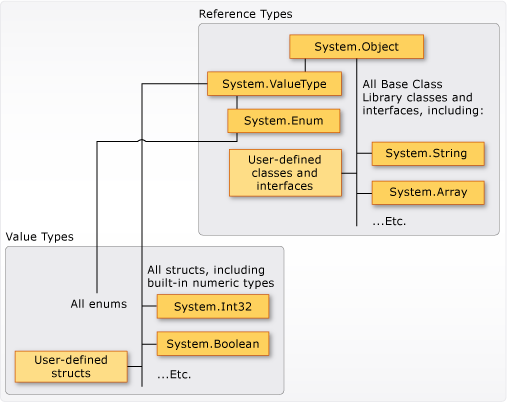
\includegraphics[width=0.7\textwidth]{bilder/value-reference-types-common-type-system.png}
		\caption{Type System in C\# \cite{progrguide}}
	\end{figure}
\end{frame}

\begin{frame}{Allgemeines Typsystem}
\begin{itemize}
% https://docs.microsoft.com/de-de/dotnet/csharp/programming-guide/types/
	\item Stark Typisiert
	\begin{itemize}
		\item jede Konstante, Variable und jeder Ausdruck hat einen Typ
	\end{itemize}
	\item CTS (Common Type System)
	\begin{itemize}
		\item \textbf{Jeder} Typ ist von \texttt{System.Object} (\texttt{object}) abgeleitet
	\end{itemize}

	\item Integrierte Typen
	\begin{itemize}
		\item \glqq Zahlen\grqq{}, \texttt{boolean}, \texttt{char}, \texttt{object}, \texttt{string}
	\end{itemize}
	\item Referenztypen / Werttypen
	\begin{itemize}
		\item \texttt{System.ValueType}
	\end{itemize}
	\item Benutzerdefinierte Typen
	\begin{itemize}
		\item \texttt{class, enum, struct}
	\end{itemize}
\end{itemize}
\end{frame}


\begin{frame}{Variablen Deklarationen}
\lstinputlisting[linerange={1-2,5-16}]{Beispielcode/variable_declaration.cs}
\begin{itemize}
	\item \texttt{var} Keyword \cite{so_var_java}
	\item LINQ
\end{itemize}
\end{frame}


\begin{frame}{Werttypen}
\lstinputlisting[linerange={6-20}]{Beispielcode/typesystem.cs}

System.Int32 \\
Int32 CompareTo(System.Object) Int32 CompareTo(Int32) ... \\
System.Int32 -> System.ValueType -> System.Object
\end{frame}


\begin{frame}{Werttypen - Vergleich Java}
	\begin{itemize}
		\item In Java: Integer $\neq$ int
		\item Zwar automatische Konvertierung, aber int ist kein Objekt
		\item Auskommentierte Zeilen führen zu Fehlern
	\end{itemize}
	\lstinputlisting[linerange={9-15}]{Beispielcode/test/test.java}
	
\end{frame}


\begin{frame}{Zusammenfassung Typen}
% Create a line splitting two columns
\setlength{\columnseprule}{0.4pt}
\begin{multicols}{2}
	Java \\
	\begin{itemize}
		\item Primitive Typen nicht von \texttt{Object} abgeleitet
		\item Call-by-Value, Call-By-Reference
		\item Wrapper-Klasse \texttt{Integer} für \texttt{int}
	\end{itemize}

\columnbreak

	C\#\\
	\begin{itemize}
		\item Alles (auch \texttt{int}) von \texttt{object} abgeleitet
		\item Zahlen, boolean sind \glqq{}Werttype\grqq{}
		\item \texttt{int} kann mit \texttt{int?} Nullable gemacht werden
	\end{itemize}
\end{multicols}
\end{frame}


\begin{frame}{Klassen}

	\begin{itemize}
		\item Erben implizit von \texttt{object}
		\item  Enthalten: \texttt{constructors}, \textbf{\texttt{properties}}, \texttt{indexers}, \texttt{events}, \texttt{operators} and \texttt{destructors}
		 \item \texttt{sealed}-Modifier: Für die gesamte Klasse oder einzelne Methoden
	\end{itemize}

\end{frame}

\begin{frame}{Vererbung}
	\lstinputlisting[basicstyle=\tiny,linerange={1-28}]{Beispielcode/classes.cs}
\end{frame}

\begin{frame}{Vererbung}
	\lstinputlisting[basicstyle=\tiny,linerange={30-41}]{Beispielcode/classes.cs}
	Base, example 1\\
	Base, example 1\\
	Derived, example 1\\
	Base, example 2\\
	Derived, example 2\\
	Derived, example 2\\
	Base, example 3\\
	Base, example 3\\
	Derived, example 3
\end{frame}

\begin{frame}{Vererbung - Vergleich Java}
	
	\begin{itemize}
		\item Java: Alle Methoden sind virtuell
		\begin{itemize}
			\item Override wird mit \texttt{final} verhindert.
			\item Kein Äquivalent zu C\# \texttt{new}
		\end{itemize}
		\item Java: \texttt{@Override} Dekorator soll Code lesbarer machen
		\item In C\# Ingesamt expliziter als in Java
		\begin{itemize}
			\item Für interessierte: Interview mit C\# Chefdesigner \cite{interview_virtual}
		\end{itemize}
	\end{itemize}

\end{frame}

\begin{frame}{Quellen}
\begin{thebibliography}{99}
\fontsize{6pt}{7.2}\selectfont
	\bibitem{progrguide}"Programming Guide C\#", \url{https://docs.microsoft.com/de-de/dotnet/csharp/programming-guide/}, 05.06.2020
	\bibitem{spec_csharp} C\# Language Specification, \url{https://docs.microsoft.com/de-de/dotnet/csharp/language-reference/language-specification/introduction}, 05.06.2020
   \bibitem{intro_csharp}Introduction to C\#, \url{https://docs.microsoft.com/de-de/dotnet/csharp/language-reference/language-specification/introduction}, 06.06.2020

 \bibitem{so_var_java}'"What is the equivalent of the C\# 'var' keyword in Java?"', 
 \url{https://stackoverflow.com/a/49598148}, 05.06.2020
 \bibitem{interview_virtual}'Interview with C\# Designer', \url{https://www.artima.com/intv/nonvirtual.html}, 06.06.2020
\end{thebibliography}
\end{frame}
\end{document}
